\documentclass{beamer}


\mode<presentation>
{
  \usetheme{CambridgeUS}
	\usecolortheme{beaver}
  % or ...

  \setbeamercovered{transparent}
  % or whatever (possibly just delete it)
}


\usepackage{xeCJK}
\usepackage{ulem}
\usepackage[english]{babel}
\usepackage[utf8]{inputenc}
\usepackage{times}
\usepackage[T1]{fontenc}
\usepackage{hyperref}
\usepackage{pifont}
\usepackage{biblatex}
\usepackage{bibentry}
\usepackage{verbatim}
\usepackage{listings}
\usepackage{subfig}
\bibliography{cite}
\newcommand{\cmark}{\ding{51}}%
\newcommand{\xmark}{\ding{55}}%
\setCJKmainfont{WenQuanYi Micro Hei}
\renewcommand{\raggedright}{\leftskip=0pt \rightskip=0pt plus 0cm}
\raggedright

\let\oldfootnotesize\footnotesize
\renewcommand*{\footnotesize}{\oldfootnotesize\tiny}

\title[Intelligent Software Engineering] 
{Intelligent Software Engineering}
\subtitle{Requirements Engineering}

\author[Zhilei Ren] 
{Zhilei Ren}

\institute[Dalian University of Technology] % (optional, but mostly needed)
{
\\
\includegraphics[width=0.1\textwidth]{../utils/logo.png}\\
Dalian University of Technology
}


\subject{Software Engineering}



\pgfdeclareimage[width=0.08\textwidth]{university-logo}{../utils/logo.png}
\logo{\pgfuseimage{university-logo}}



% Delete this, if you do not want the table of contents to pop up at
% the beginning of each subsection:
\AtBeginSubsection[]
{
  \begin{frame}<beamer>{Outline}
    \tableofcontents[currentsection,currentsubsection]
  \end{frame}
}


% If you wish to uncover everything in a step-wise fashion, uncomment
% the following command: 

%\beamerdefaultoverlayspecification{<+->}

\setbeamertemplate{section in toc}[circle]
\setbeamertemplate{items}[circle]
\setbeamertemplate{caption}[numbered]
\setbeamertemplate{bibliography item}{\insertbiblabel}
\setbeamertemplate{bibliography entry title}{}
\setbeamertemplate{bibliography entry journal}{}

% PlantUML listing configuration
\lstdefinestyle{plantuml}{
    language=Java,
    basicstyle=\ttfamily\small,
    keywordstyle=\color{blue},
    commentstyle=\color{green!60!black},
    stringstyle=\color{red},
    numbers=left,
    numberstyle=\tiny\color{gray},
    stepnumber=1,
    numbersep=5pt,
    backgroundcolor=\color{white!95!black},
    frame=single,
    rulecolor=\color{black},
    tabsize=2,
    captionpos=b,
    breaklines=true,
    breakatwhitespace=false,
    showstringspaces=false,
    basicstyle=\ttfamily\footnotesize,
}
% \lstset{basicstyle=\footnotesize,}
\lstdefinestyle{code}{
    basicstyle=\ttfamily\tiny,
    backgroundcolor=\color{white!95!black},
    frame=single,
    rulecolor=\color{black},
    breaklines=true,
    captionpos=b
}

\begin{document}

\begin{frame}
  \titlepage
\end{frame}

%\begin{frame}{Outline}
%  \tableofcontents[currentsection,currentsubsection, 
%    hideothersubsections, 
%    sectionstyle=show,
%]
%\end{frame}

\AtBeginSection[]
{
 \begin{frame}<beamer>
 \frametitle{Outline}
 \tableofcontents[currentsection]
 \end{frame}
}
\section{Introduction}
\begin{frame}[t]{Definition of Requirements Engineering}
    Requirements engineering is an interdisciplinary function that mediates between the domains of the acquirer and supplier or developer to establish and maintain the requirements to be met by the system, software or service of interest. Requirements engineering is concerned with discovering, eliciting, developing, analyzing, verifying (including verification methods and strategy), validating, communicating, documenting and managing requirements\footnote{ISO/IEC/IEEE 29148 Systems and software engineering — Life cycle processes -- Requirements engineering}.
\end{frame}

\begin{frame}[t]{As Proposed by the Project Sponsor}
    \centering
    
\includegraphics[width=.4\textwidth]{treemark.jpg} 
\end{frame}

\begin{frame}[t]{As Specified in the Project Request}
    \centering
    
\includegraphics[width=.4\textwidth]{treemana.jpg} 
\end{frame}
\begin{frame}[t]{As Designed by the Senior Systems Analyst}
    \centering
    
\includegraphics[width=.4\textwidth]{treeeng.jpg} 
\end{frame}
\begin{frame}[t]{As Produced by the Programmers}
    \centering
    
\includegraphics[width=.4\textwidth]{treemanu.jpg} 
\end{frame}
\begin{frame}[t]{As Installed at the User's Site}
    \centering
    
\includegraphics[width=.4\textwidth]{treemain.jpg} 
\end{frame}
\begin{frame}[t]{What The User Wanted}
    \centering
    
\includegraphics[width=.4\textwidth]{treecust.jpg}
\end{frame}

\begin{frame}[t]{Guide to Good Programming Practice, 1979}
    \centering
    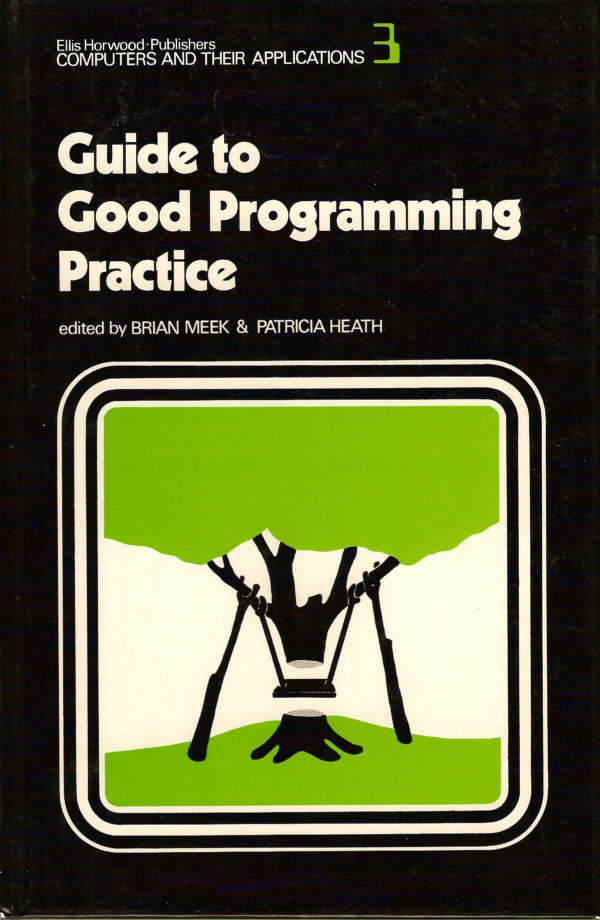
\includegraphics[width=.4\textwidth]{treeswing_computer_book_cover.jpg}
\end{frame}

\begin{frame}[t]{bug or feature?}
    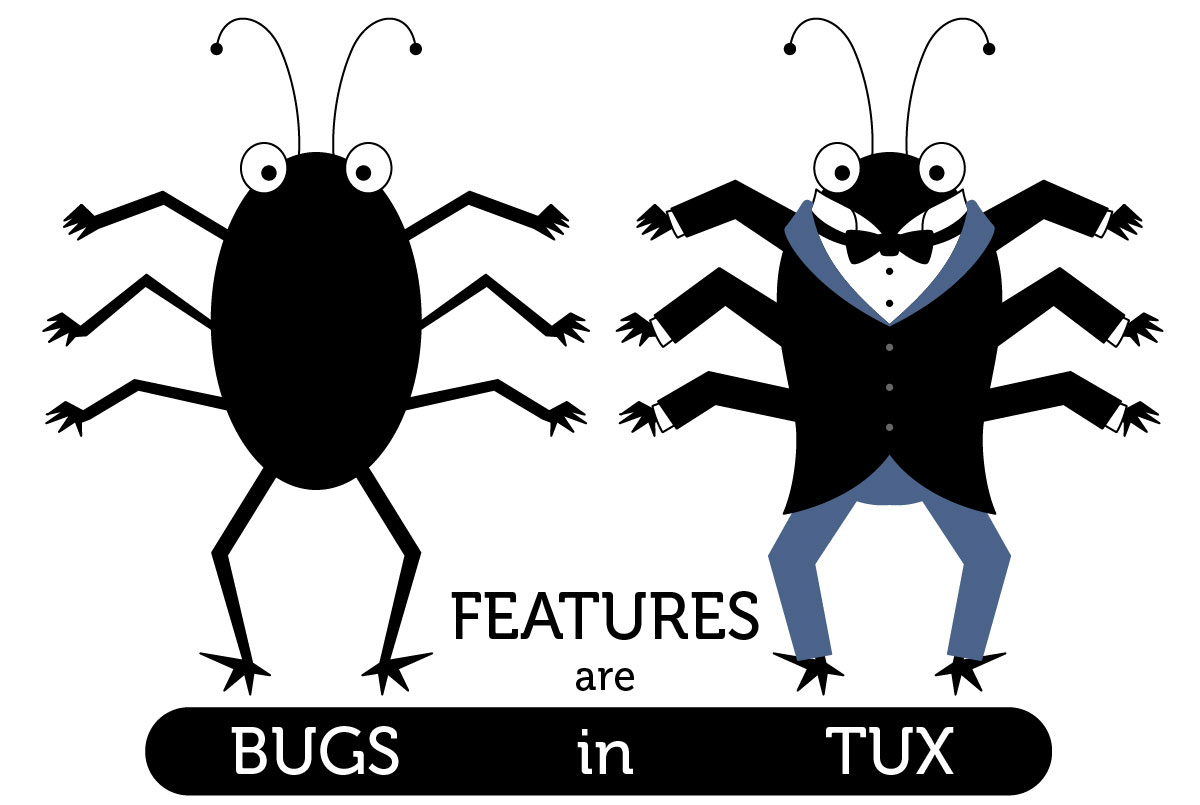
\includegraphics[width=.5\textwidth]{bugfeature.jpg}
\end{frame}
\begin{frame}[t]{The First Computer Bug}
    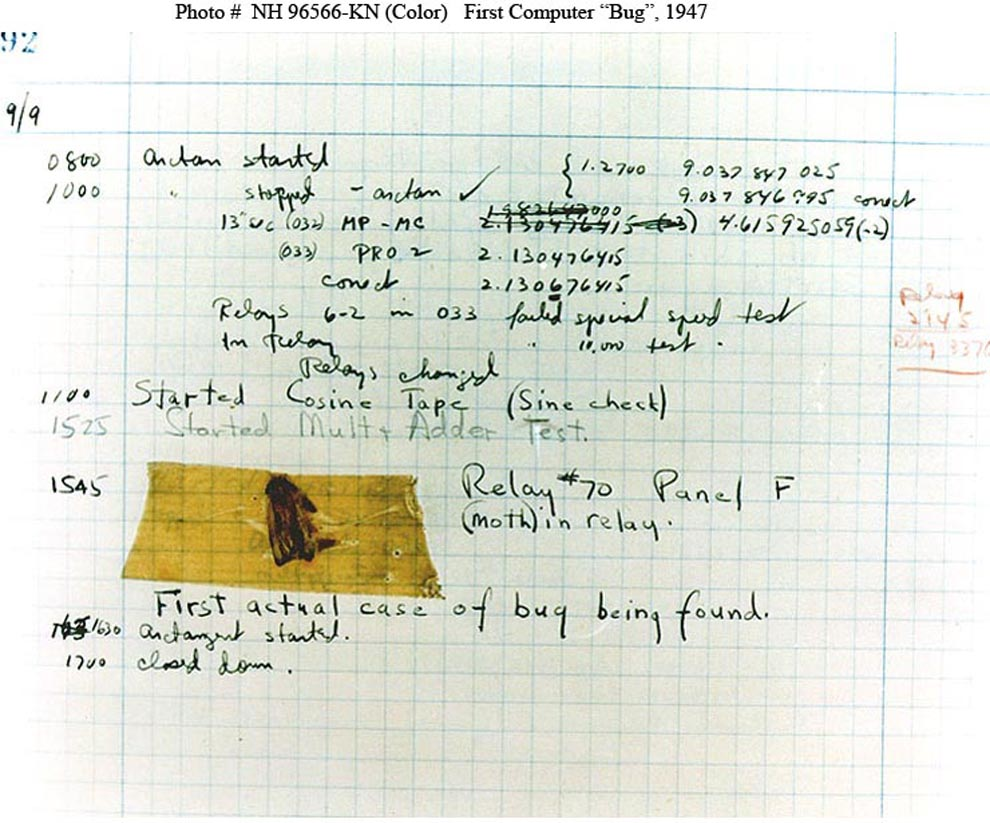
\includegraphics[width=.5\textwidth]{computer-bug.jpg}  
\end{frame}
\begin{frame}[t]{The First Computer Bug}
    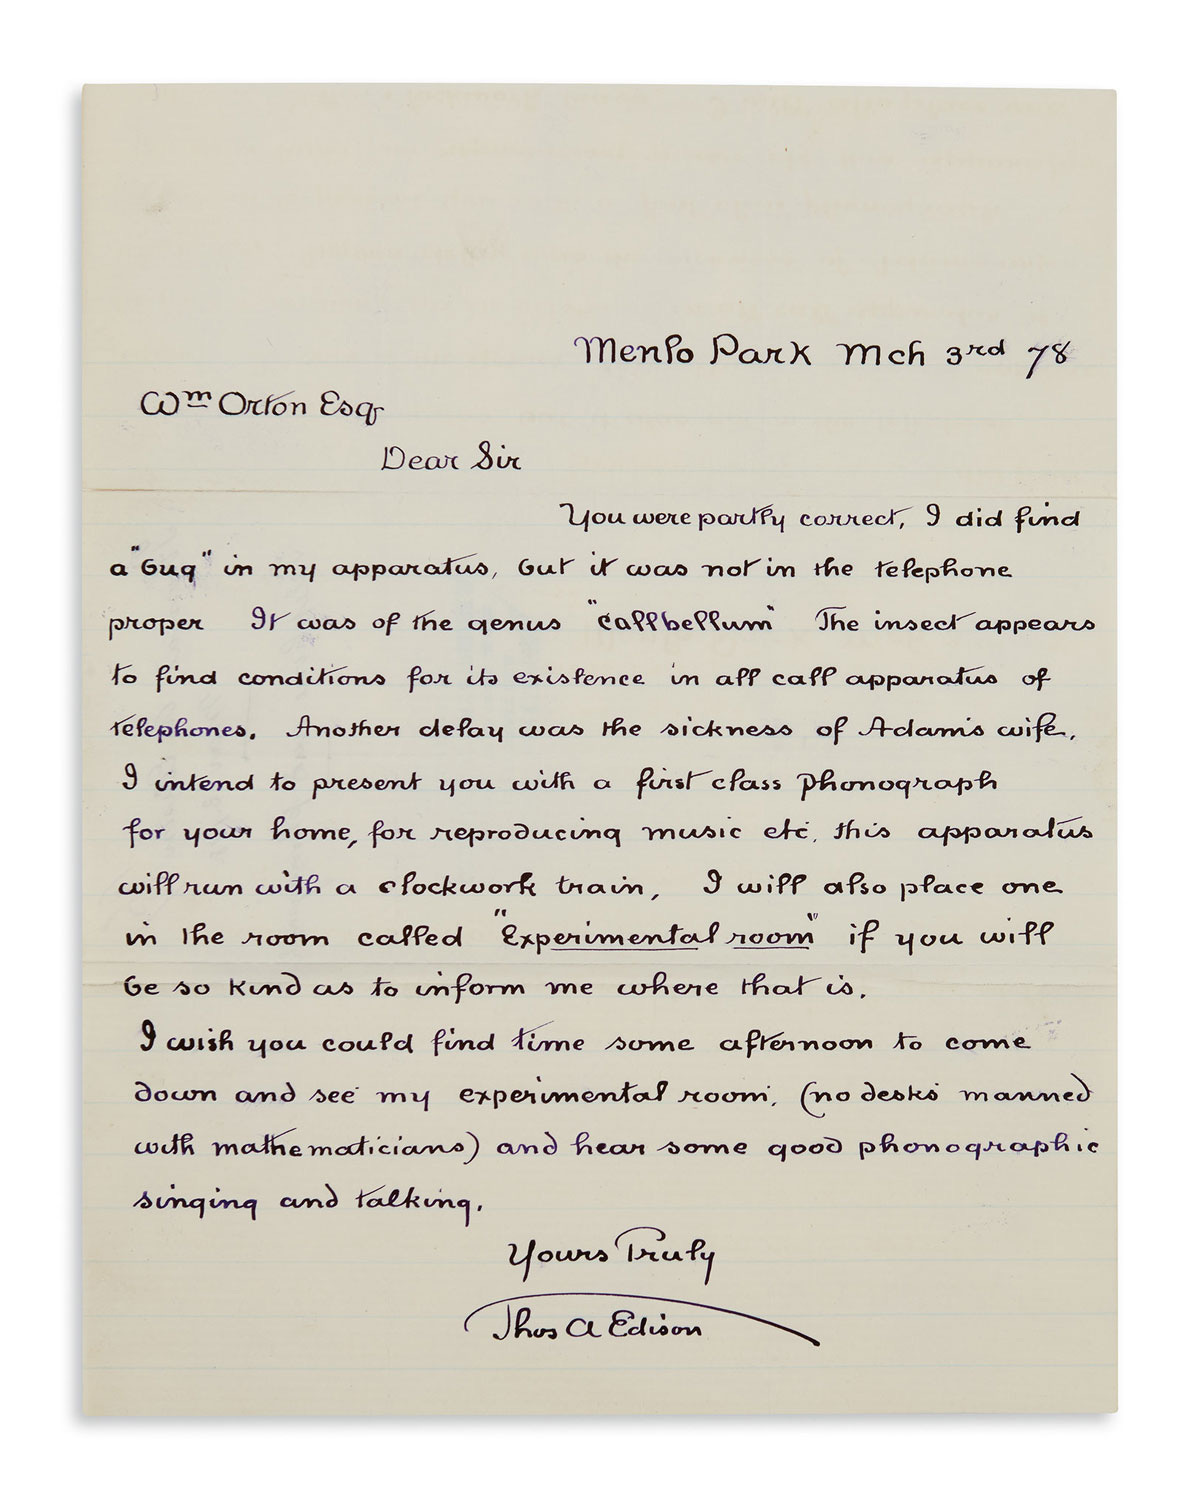
\includegraphics[width=.5\textwidth]{telebug.jpg}  
\end{frame}
\begin{frame}[t]{Combo in Fighting Games was originally a Bug}
    Combos were a design accident; lead producer Noritaka Funamizu noticed that extra strikes were possible during a bug check on the car-smashing bonus stage. He thought that the timing required was too difficult to make it a useful game feature, but left it in as a hidden one\footnote{\url{https://en.wikipedia.org/wiki/Combo_(video_games)}}.

    \begin{figure}
    \begin{center}
    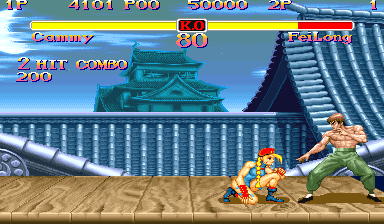
\includegraphics[width=.5\textwidth]{Super_Street_Fighter_II_screenshot.png}
    \end{center}
    \caption{Street Fighter 2}
    \label{fig:}
    \end{figure}

\end{frame}

\begin{frame}{Hidden Features aka Easter Egg}
    \begin{figure}
    \begin{center}
        
\includegraphics[width=.5\textwidth]{images/1280px-Konami_Code.svg.png}
    \end{center}
    \caption{The Konami Code}
    \label{fig:konami}
    \end{figure}

    Finding the game too difficult to play through during testing, he (Konami developer) created the cheat code, which gives the player a full set of power-ups\ldots The code was meant to be removed prior to publishing, but this was overlooked and only discovered as the game was being prepared for mass production. The developers decided to leave it there, as removing it could result in new bugs and glitches\footnote{\url{https://en.wikipedia.org/wiki/Konami_Code}}. 
\end{frame}

\begin{frame}{Be Careful with Putting Easter Egg in Software}
        \begin{figure}[b]
        \centering
        \subfloat[Test Failure due to man]{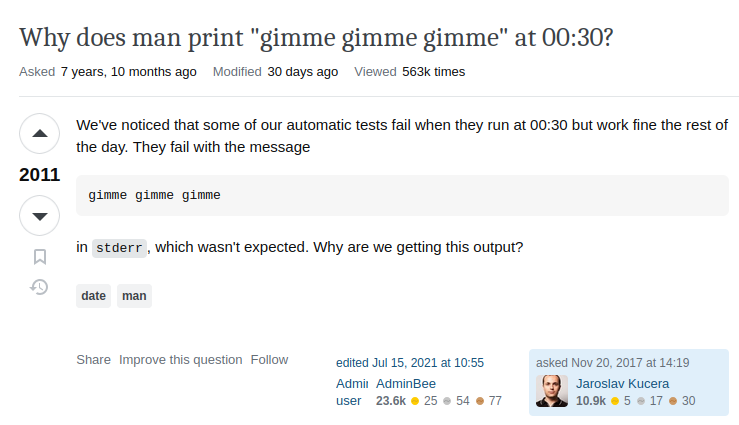
\includegraphics[width=5cm]{images/test_failure.png}}\qquad    
        \subfloat[The Root Cause]{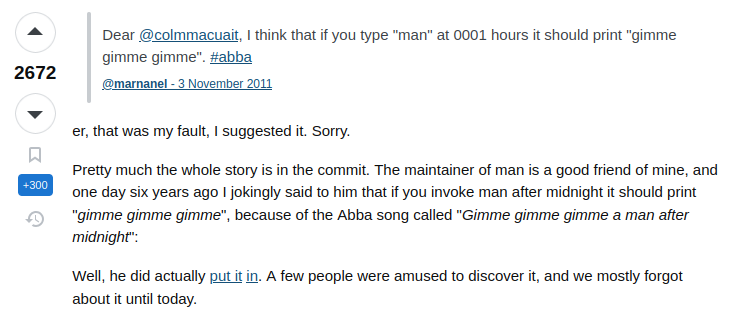
\includegraphics[width=5cm]{images/gimme.png}}    


        \caption{Bug Caused by an Easter Egg}
        \end{figure}
    
    

    
\end{frame}

\section{Assisting Requirements Engineering with LLM}

\begin{frame}{What is Requirements Engineering?}
    \begin{block}{Definition}
        Requirements Engineering (RE) is the process of defining, documenting, and maintaining requirements in the engineering design process.
    \end{block}
    
    \begin{itemize}
        \item \textbf{Elicitation}: Discovering requirements from stakeholders
        \item \textbf{Analysis}: Refining and modeling requirements
        \item \textbf{Specification}: Documenting requirements unambiguously
        \item \textbf{Validation}: Ensuring requirements meet stakeholder needs
        \item \textbf{Management}: Managing requirements changes throughout project lifecycle
    \end{itemize}
\end{frame}

\begin{frame}{Traditional RE Challenges}
    \begin{columns}
        \begin{column}{0.5\textwidth}
            \textbf{Common Issues:}
            \begin{itemize}
                \item Incomplete requirements
                \item Changing requirements
                \item Communication gaps
                \item Ambiguous specifications
                \item Stakeholder conflicts
            \end{itemize}
        \end{column}
        \begin{column}{0.5\textwidth}
            \centering
            \includegraphics[width=0.8\textwidth]{example-image} % Placeholder
        \end{column}
    \end{columns}
\end{frame}

% Slide 1: What is PlantUML?
\begin{frame}{What is PlantUML?}
    \begin{itemize}
        \item \textbf{Core Idea:} Uses simple, human-readable Domain Specific Language (DSL)
        \item \textbf{Foundation:} Java-based tool for layout
        \item \textbf{Philosophy:} Focus on content rather than manual layout
    \end{itemize}
    
    \begin{quote}
        "PlantUML is a versatile component for quickly and directly creating diagrams."
    \end{quote}
\end{frame}

% Slide 2: Key Advantages
\begin{frame}{Key Advantages}
    \begin{table}
    \small
    \begin{tabular}{p{0.4\textwidth} p{0.55\textwidth}}
    \textbf{Advantage} & \textbf{Description} \\
    \hline
    Version Control Friendly & Text files work with Git - enables change history, diffing, collaboration \\
    Efficiency \& Speed & Faster than manual graphical editing, especially for complex diagrams \\
    Maintainability \& Consistency & Easy updates and consistent styling with themes \\
    Automation \& Integration & Integrates with documentation pipelines, build systems, CI/CD \\
    \end{tabular}
    \end{table}
\end{frame}

% Slide 3: UML Diagrams Supported
\begin{frame}{UML Diagrams Supported}
    \begin{columns}
    \begin{column}{0.5\textwidth}
        \begin{itemize}
            \item Sequence Diagram
            \item Use Case Diagram
            \item Class Diagram
            \item Activity Diagram
            \item Component Diagram
            \item Deployment Diagram
            \item State Diagram
            \item Object Diagram
        \end{itemize}
    \end{column}
    \begin{column}{0.5\textwidth}
        \centering
        \textbf{Visual Example:}\\
        \textcolor{gray}{\scriptsize[Diagram placeholder]}
        \vspace{2cm}
    \end{column}
    \end{columns}
\end{frame}

% Slide 4: Beyond UML
\begin{frame}{Beyond UML Diagrams}
    \begin{itemize}
        \item Architectural Diagrams (C4 model)
        \item Entity Relationship Diagrams (ERD)
        \item Wireframes / UI Mockups (salt library)
        \item Gantt charts for project management
        \item Mind Maps for brainstorming
        \item JSON/YAML visualization
        \item Network diagrams
    \end{itemize}
\end{frame}

% Slide 5: How It Works
\begin{frame}{How PlantUML Works}
    \begin{enumerate}
        \item \textbf{Write:} Create text file (.puml) with PlantUML syntax
        \item \textbf{Process:} Java processor parses text
        \item \textbf{Render:} Layout engine generates final image
        \item \textbf{Output:} Get image in desired format (PNG, SVG, etc.)
    \end{enumerate}
    
    \begin{center}
    \textbf{Text} $\rightarrow$ \textbf{PlantUML} $\rightarrow$ \textbf{Diagram}
    \end{center}
\end{frame}

% Slide 6: Sequence Diagram Example
\begin{frame}[fragile,t]{Syntax Example: Sequence Diagram}
    \begin{lstlisting}[style=plantuml]
@startuml
actor User
participant "Web Browser" as Browser
participant Server

autonumber
User -> Browser: Enter URL
Browser -> Server: HTTP Request
Server -> Server: Process Request
Server --> Browser: Return HTML
Browser --> User: Display Page
@enduml
    \end{lstlisting}

    
    
    \small
    \begin{itemize}
        \item \texttt{@startuml/@enduml}: Diagram boundaries
        \item \texttt{actor}, \texttt{participant}: Element declarations
        \item \texttt{->}, \texttt{-{}->}: Solid/dashed arrows
        \item \texttt{autonumber}: Automatic message numbering
    \end{itemize}
\end{frame}

\begin{frame}[fragile,t]{Syntax Example: Sequence Diagram}
    \begin{lstlisting}[style=plantuml]
@startuml
actor User
participant "Web Browser" as Browser
participant Server

autonumber
User -> Browser: Enter URL
Browser -> Server: HTTP Request
Server -> Server: Process Request
Server --> Browser: Return HTML
Browser --> User: Display Page
@enduml
    \end{lstlisting}
    
    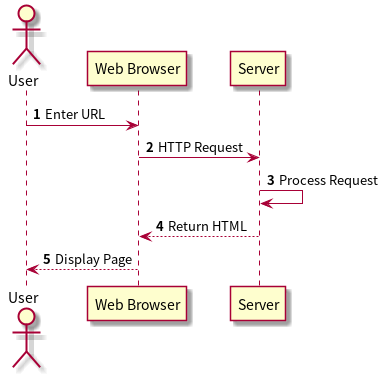
\includegraphics[width=.3\textwidth]{images/sequence.png} 
\end{frame}

% Slide 7: Use Case Diagram Example
\begin{frame}[fragile,t]{Syntax Example: Use Case Diagram}
    \begin{lstlisting}[style=plantuml]
@startuml
left to right direction
actor "Library User" as User
usecase "Borrow Book" as Borrow
usecase "Search Catalog" as Search

User --> Borrow
User --> Search
@enduml
    \end{lstlisting}
    
    \small
    \begin{itemize}
        \item \texttt{left to right direction}: Layout control
        \item \texttt{actor}, \texttt{usecase}: Actor and use case definitions
        \item \texttt{-->}: Connection arrows
    \end{itemize}
\end{frame}

% Slide 7: Use Case Diagram Example
\begin{frame}[fragile,t]{Syntax Example: Use Case Diagram}
    \begin{lstlisting}[style=plantuml]
@startuml
left to right direction
actor "Library User" as User
usecase "Borrow Book" as Borrow
usecase "Search Catalog" as Search

User --> Borrow
User --> Search
@enduml
    \end{lstlisting}
    
    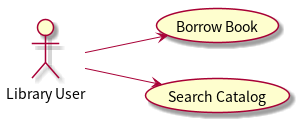
\includegraphics[width=.3\textwidth]{images/usecase.png} 
\end{frame}

% Slide 8: Getting Started
\begin{frame}{Getting Started with PlantUML}
    \textbf{Online Servers (Quick Start):}
    \begin{itemize}
        \item Official server: \href{http://plantuml.com}{plantuml.com}
        \item Community site: \href{http://planttext.com}{planttext.com}
        \item No installation required
    \end{itemize}
    
    \vspace{0.5cm}
    \textbf{Local Installation (Recommended):}
    \begin{itemize}
        \item Prerequisites: Java JRE + Graphviz
        \item IDE Plugins: VSCode, IntelliJ, Eclipse
        \item Command Line: Use \texttt{plantuml.jar}
    \end{itemize}
\end{frame}

% Slide 9: Summary
\begin{frame}{Summary \& Key Takeaways}
    \begin{itemize}
        \item \textbf{Why PlantUML?} Version control, automation, efficiency
        \item \textbf{Text-Based:} Simple, readable language for diagrams
        \item \textbf{Wide Support:} Comprehensive UML + additional diagram types
        \item \textbf{Easy Integration:} Fits modern development workflows
        \item \textbf{Quick Start:} Online editors → local integration
    \end{itemize}
    
    \vspace{0.5cm}
    \textbf{Embrace efficient diagram creation and maintenance!}
\end{frame}

\begin{frame}{What is Prompt Engineering?}
    \begin{block}{Definition}
        Prompt Engineering is the practice of designing and optimizing inputs (prompts) to effectively communicate with AI models to generate desired outputs.
    \end{block}
    
    \begin{itemize}
        \item \textbf{Precision}: Crafting clear, specific instructions
        \item \textbf{Context}: Providing relevant background information
        \item \textbf{Structure}: Organizing information logically
        \item \textbf{Iteration}: Refining based on model responses
        \item \textbf{Validation}: Ensuring output meets requirements
    \end{itemize}
\end{frame}

\begin{frame}{Prompt Engineering Techniques}
    \begin{columns}
        \begin{column}{0.6\textwidth}
            \textbf{Key Techniques:}
            \begin{itemize}
                \item Zero-shot vs. Few-shot prompting
                \item Chain-of-Thought reasoning
                \item Role-playing scenarios
                \item Template-based prompts
                \item Iterative refinement
            \end{itemize}
        \end{column}
        \begin{column}{0.4\textwidth}
            \centering
            \includegraphics[width=0.8\textwidth]{example-image} % Placeholder
        \end{column}
    \end{columns}
\end{frame}

\begin{frame}{Zero-shot vs. Few-shot Prompting}
    \begin{block}{Zero-shot Prompting}
        Providing no examples - the model must understand and respond based solely on the instruction
    \end{block}
    
    \begin{exampleblock}{RE Example - Zero-shot}
        \texttt{"Generate functional requirements for a user login system"}
    \end{exampleblock}
    
    \begin{block}{Few-shot Prompting}
        Providing several examples to demonstrate the desired pattern or format
    \end{block}
    
    \begin{exampleblock}{RE Example - Few-shot}
        \texttt{"Here are examples of good requirements: \\1. The system shall validate user credentials\\2. The system shall encrypt passwords\\ Now generate requirements for user registration"}
    \end{exampleblock}
\end{frame}

\begin{frame}[fragile]{Zero-shot vs. Few-shot: Practical Examples}
    \begin{columns}
        \begin{column}{0.5\textwidth}
            \textbf{Zero-shot Example:}
            \begin{lstlisting}[style=code]
Create a use case for 
"password reset" functionality
            \end{lstlisting}
            
            \textbf{Pros:}
            \begin{itemize}
                \item Quick and simple
                \item Good for straightforward tasks
                \item Less context needed
            \end{itemize}
        \end{column}
        \begin{column}{0.5\textwidth}
            \textbf{Few-shot Example:}
            \begin{lstlisting}[style=code]
Example 1: Use case for login
- Actor: User
- Precondition: Valid account
- Steps: Enter credentials...

Example 2: Use case for logout
- Actor: User
- Precondition: Logged in
- Steps: Click logout...

Now create for "password reset"
            \end{lstlisting}
            
            \textbf{Pros:}
            \begin{itemize}
                \item Better quality output
                \item Consistent formatting
                \item Handles complex patterns
            \end{itemize}
        \end{column}
    \end{columns}
\end{frame}

\begin{frame}{Chain-of-Thought Reasoning}
    \begin{block}{Definition}
        Breaking down complex problems into intermediate reasoning steps, mimicking human problem-solving
    \end{block}
    
    \begin{exampleblock}{RE Application}
        Instead of asking for complete requirements, guide the AI through logical steps:
        \begin{enumerate}
            \item Identify stakeholders
            \item Define high-level goals
            \item Break down into features
            \item Specify detailed requirements
            \item Validate completeness
        \end{enumerate}
    \end{exampleblock}
    
    \textbf{Benefits for Requirements Engineering:}
    \begin{itemize}
        \item Reduces ambiguity in complex domains
        \item Ensures logical consistency
        \item Helps identify missing requirements
        \item Improves traceability
    \end{itemize}
\end{frame}

\begin{frame}[fragile]{Chain-of-Thought: Requirements Example}
    \begin{lstlisting}[style=code, caption={Chain-of-Thought for Payment System}]
Let's design requirements for an online payment system:

Step 1: Identify main stakeholders
- Customers, merchants, payment processors, banks

Step 2: Define core functionality needed
- Payment processing, security, fraud detection

Step 3: For payment processing, consider:
- Payment methods (credit card, digital wallets)
- Transaction flow (initiation, validation, completion)
- Error handling (declined payments, timeouts)

Step 4: Security requirements:
- Data encryption, PCI compliance, authentication

Step 5: Now generate detailed functional requirements 
for the payment processing component...
    \end{lstlisting}
\end{frame}

\begin{frame}{Role-playing Scenarios}
    \begin{block}{Concept}
        Asking the AI to adopt a specific persona or role to generate more context-appropriate responses
    \end{block}
    
    \begin{exampleblock}{RE Roles Examples}
        \begin{itemize}
            \item \textbf{Product Owner}: "Act as a product owner for an e-commerce platform..."
            \item \textbf{System Architect}: "You are a system architect designing a microservices architecture..."
            \item \textbf{Quality Assurance Engineer}: "As a QA engineer, create test scenarios for..."
            \item \textbf{End User}: "From the perspective of a novice user, what features would you need..."
        \end{itemize}
    \end{exampleblock}
    
    \textbf{Advantages:}
    \begin{itemize}
        \item Generates perspective-specific requirements
        \item Identifies conflicting needs early
        \item Improves requirement completeness
    \end{itemize}
\end{frame}

\begin{frame}[fragile]{Role-playing in Requirements Elicitation}
    \begin{columns}
        \begin{column}{0.5\textwidth}
            \textbf{Without Role-playing:}
            \begin{lstlisting}[style=code]
List requirements for 
a project management tool
            \end{lstlisting}
        \end{column}
        \begin{column}{0.5\textwidth}
            \textbf{With Role-playing:}
            \begin{lstlisting}[style=code]
Act as a project manager with 
10 years experience in agile 
environments. What requirements 
would you prioritize for a 
project management tool?
            \end{lstlisting}
        \end{column}
    \end{columns}
    
    \vspace{0.5cm}
    \textbf{Specific Role Examples:}
    
    \begin{lstlisting}[style=code]
Role: Security Auditor
"Identify security requirements for a healthcare app handling patient data, considering HIPAA compliance"

Role: Accessibility Specialist  
"Generate accessibility requirements for a banking application to ensure WCAG 2.1 AA compliance"
    \end{lstlisting}
\end{frame}

\begin{frame}{Template-based Prompts}
    \begin{block}{Definition}
        Using structured templates to ensure consistent, comprehensive outputs across different requirements
    \end{block}
    
    \textbf{Common RE Templates:}
    \begin{itemize}
        \item Use Case Template
        \item User Story Template
        \item Functional Requirement Template
        \item Non-functional Requirement Template
        \item Acceptance Criteria Template
    \end{itemize}
    
    \begin{exampleblock}{Benefits}
        \begin{itemize}
            \item Standardized format across the project
        \item Easier validation and review
        \item Better integration with RE tools
        \item Consistent quality of generated content
        \end{itemize}
    \end{exampleblock}
\end{frame}

\begin{frame}[fragile]{Template Examples for Requirements Engineering}
    \begin{lstlisting}[style=code, caption={Use Case Template}]
USE CASE TEMPLATE:
[System Name] - [Use Case Name]

ID: [Unique Identifier]
Primary Actor: [Role]
Secondary Actors: [Optional Roles]

Preconditions:
- [Condition 1]
- [Condition 2]

Main Success Scenario:
1. [Step 1]
2. [Step 2]
3. [Step 3]

Alternative Flows:
- [A1]: [Description]
- [A2]: [Description]

Postconditions:
- [State 1]
- [State 2]

Exceptions:
- [E1]: [Error condition]
    \end{lstlisting}
\end{frame}

\begin{frame}[fragile]{Functional Requirements Template}
    \begin{lstlisting}[style=code, caption={Structured Requirements Template}]
REQUIREMENT TEMPLATE:

Requirement ID: [FR-001]
Type: [Functional/Non-functional]
Priority: [High/Medium/Low]

Description: 
[Clear, unambiguous description of what the system shall do]

Source:
[Stakeholder/Business Need/Regulation]

Rationale:
[Why this requirement is needed]

Acceptance Criteria:
1. [Criterion 1 - testable condition]
2. [Criterion 2 - testable condition]
3. [Criterion 3 - testable condition]

Dependencies:
- [Related requirement IDs]

Constraints:
- [Technical/business constraints]

Status: [Proposed/Approved/Implemented]
    \end{lstlisting}
\end{frame}

\begin{frame}{Iterative Refinement}
    \begin{block}{Concept}
        Starting with broad requirements and progressively refining them through multiple iterations of feedback and clarification
    \end{block}
    
    \textbf{Iterative Process:}
    \begin{enumerate}
        \item \textbf{First Pass}: High-level requirements and scope
        \item \textbf{Second Pass}: Detailed functional requirements
        \item \textbf{Third Pass}: Non-functional requirements and constraints
        \item \textbf{Final Pass}: Validation and acceptance criteria
    \end{enumerate}
    
    \begin{exampleblock}{RE Application}
        \begin{itemize}
            \item Start with epic-level user stories
            \item Break down into features
            \item Refine into detailed user stories
            \item Add technical specifications
            \item Validate with stakeholders
        \end{itemize}
    \end{exampleblock}
\end{frame}

\begin{frame}[fragile]{Iterative Refinement Example}
    \begin{columns}
        \begin{column}{0.5\textwidth}
            \textbf{Iteration 1: High-level}
            \begin{lstlisting}[style=code]
Create requirements for 
user authentication system
            \end{lstlisting}
        \end{column}
        \begin{column}{0.5\textwidth}
            \textbf{Iteration 2: More specific}
            \begin{lstlisting}[style=code]
Add multi-factor 
authentication support
            \end{lstlisting}
        \end{column}
    \end{columns}
    
    \vspace{0.3cm}
    \begin{columns}
        \begin{column}{0.5\textwidth}
            \textbf{Iteration 3: Detailed}
            \begin{lstlisting}[style=code]
Specify timeout policies 
and password complexity rules
            \end{lstlisting}
        \end{column}
        \begin{column}{0.5\textwidth}
            \textbf{Iteration 4: Validation}
            \begin{lstlisting}[style=code]
Add error handling for 
failed authentication attempts
            \end{lstlisting}
        \end{column}
    \end{columns}
    
    \vspace{0.5cm}
    \textbf{Benefits of Iterative Approach:}
    \begin{itemize}
        \item Catches ambiguities early
        \item Allows for stakeholder feedback at each stage
        \item Reduces rework
        \item Builds comprehensive requirement sets
    \end{itemize}
\end{frame}

\begin{frame}[fragile]{Complete Iterative Refinement Workflow}
    \begin{lstlisting}[style=code, caption={Multi-stage Refinement Process}]
// Stage 1: Scope Definition
"Define the high-level scope for a customer relationship management system"

// Stage 2: Feature Identification  
"Based on the scope, identify key features needed for lead management"

// Stage 3: Detailed Requirements
"For the lead management feature, specify functional requirements including lead capture, assignment, and tracking"

// Stage 4: Validation Criteria
"Add acceptance criteria and test scenarios for lead assignment functionality"

// Stage 5: Edge Cases
"Identify and specify requirements for edge cases like duplicate lead detection and lead expiration"
    \end{lstlisting}
\end{frame}

\begin{frame}{Technique Selection Guide}
    \begin{table}
        \scriptsize
        \centering
        \begin{tabular}{p{0.25\textwidth}|p{0.3\textwidth}|p{0.3\textwidth}}
            \textbf{Technique} & \textbf{Best For} & \textbf{RE Phase} \\
            \hline
            Zero-shot & Simple, well-understood requirements & Initial scoping \\
            Few-shot & Consistent formatting, complex patterns & Detailed specification \\
            Chain-of-Thought & Complex domains, logical decomposition & Analysis and modeling \\
            Role-playing & Stakeholder perspective, conflict resolution & Elicitation and validation \\
            Template-based & Standardization, tool integration & Specification and documentation \\
            Iterative refinement & Complex systems, evolving requirements & All phases, especially management \\
        \end{tabular}
        \caption{Selecting the Right Prompt Engineering Technique}
    \end{table}
    
    \textbf{Combination Approach:}
    \scriptsize
    \begin{itemize}
        \item Start with role-playing for stakeholder perspective
        \item Use chain-of-thought for complex analysis
        \item Apply templates for consistent documentation
        \item Iterate based on feedback
    \end{itemize}
\end{frame}

\begin{frame}{Case Study: Applying Multiple Techniques}
    \begin{block}{Scenario: Healthcare Patient Portal}
        Developing requirements for a secure patient portal with medical records access
    \end{block}
    
    \textbf{Applied Techniques:}
    \begin{enumerate}
        \item \textbf{Role-playing}: "Act as a healthcare compliance officer concerned with HIPAA"
        \item \textbf{Chain-of-Thought}: Break down security requirements step by step
        \item \textbf{Template-based}: Use standardized requirement templates
        \item \textbf{Few-shot}: Provide examples of good medical software requirements
        \item \textbf{Iterative refinement}: Multiple rounds of stakeholder review
    \end{enumerate}
    
    \textbf{Results:}
    \begin{itemize}
        \item 30\% more comprehensive security requirements
        \item Early identification of compliance gaps
        \item Consistent documentation format
        \item Higher stakeholder satisfaction
    \end{itemize}
\end{frame}

\begin{frame}{Summary: Prompt Engineering for RE}
            \textbf{Key Takeaways:}
            \begin{itemize}
                \item Different techniques serve different RE needs
                \item Techniques can and should be combined
                \item Start simple, add complexity as needed
                \item Always validate AI-generated requirements
                \item Document your prompt strategies for reproducibility
            \end{itemize}
    
    \vspace{0.5cm}
    \textbf{Next Steps:}
    \begin{itemize}
        \item Practice each technique with sample RE scenarios
        \item Develop organizational prompt templates
        \item Establish validation processes for AI-generated content
        \item Integrate with existing RE workflows
    \end{itemize}
\end{frame}

\section{Bridging RE and Prompt Engineering}

\begin{frame}{Parallels Between RE and Prompt Engineering}
    \begin{table}
        \centering
        \begin{tabular}{p{0.45\textwidth}|p{0.45\textwidth}}
            \textbf{Requirements Engineering} & \textbf{Prompt Engineering} \\
            \hline
            Stakeholder needs analysis & Understanding user intent \\
            Requirements elicitation & Prompt design and formulation \\
            Use case modeling & Scenario specification \\
            Requirements specification & Clear instruction crafting \\
            Validation and verification & Output evaluation and refinement \\
            Change management & Prompt iteration \\
        \end{tabular}
        \caption{Comparative Analysis}
    \end{table}
\end{frame}

\begin{frame}{AI-Assisted Requirements Engineering}
    \begin{block}{The New Paradigm}
        Using prompt engineering techniques to enhance traditional requirements engineering processes
    \end{block}
    
    \begin{itemize}
        \item \textbf{Automated Requirements Generation}: AI can help draft initial requirements
        \item \textbf{Requirements Analysis}: AI can identify inconsistencies and gaps
        \item \textbf{Use Case Development}: AI can generate and refine use cases
        \item \textbf{Specification Writing}: AI can help create clear, unambiguous specifications
        \item \textbf{Validation Support}: AI can simulate scenarios and identify edge cases
    \end{itemize}
\end{frame}

\section{Use Case Example with PlantUML}

\begin{frame}[fragile]{Sample Prompt for Use Case Generation}
    \begin{block}{Effective Prompt Structure}
        \lstset{style=code}
        \begin{lstlisting}
Act as a requirements engineer. Generate a use case 
diagram for an online banking system including: 
authentication, balance check, funds transfer, and 
transaction history. Use PlantUML syntax.
        \end{lstlisting}
    \end{block}
    
    \begin{itemize}
        \item \textbf{Role specification}: "Act as a requirements engineer"
        \item \textbf{Context}: "online banking system"
        \item \textbf{Specific requirements}: listed functionalities
        \item \textbf{Format specification}: "Use PlantUML syntax"
    \end{itemize}
\end{frame}

\begin{frame}[fragile]{Generated Use Case Diagram (PlantUML Code)}
    \lstset{style=plantuml}
    \begin{lstlisting}[caption={Online Banking System Use Case Diagram}, label={lst:usecase}]
@startuml
left to right direction
actor "Bank Customer" as Customer
actor "Bank Manager" as Manager
actor "System Administrator" as Admin

rectangle "Online Banking System" {
    usecase "Authenticate User" as UC1
    usecase "Check Balance" as UC2
    usecase "Transfer Funds" as UC3
    usecase "View Transaction History" as UC4
    usecase "Generate Reports" as UC5
    usecase "Manage Users" as UC6
}
Customer --> UC1
Customer --> UC2
Customer --> UC3
Customer --> UC4
Manager --> UC1
Manager --> UC4
Manager --> UC5
Admin --> UC1
Admin --> UC6
UC1 .> UC2 : <<include>>
UC1 .> UC3 : <<include>>
UC1 .> UC4 : <<include>>
@enduml
    \end{lstlisting}
\end{frame}

\begin{frame}{Expected Use Case Diagram Output}
    \begin{center}
        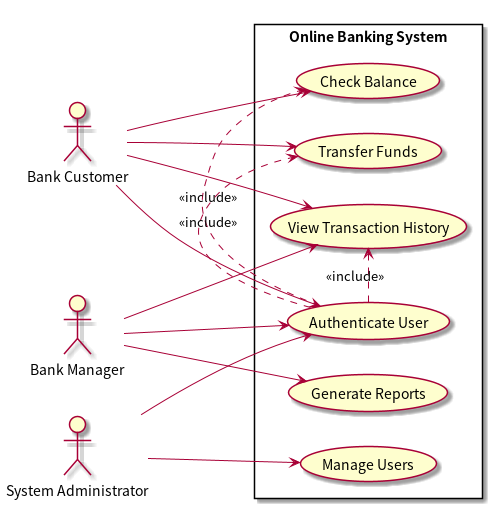
\includegraphics[width=0.4\textwidth]{images/uc.png} % Placeholder for PlantUML diagram
    \end{center}
    
    \textbf{Key Components:}
    \begin{itemize}
        \item Actors: Customer, Manager, Administrator
        \item Use Cases: Authentication, Balance Check, Funds Transfer, etc.
        \item Relationships: Associations and <<include>> dependencies
    \end{itemize}
\end{frame}

\begin{frame}[fragile]{Use Case Specification Prompt}
    \begin{block}{Detailed Use Case Prompt}
        \lstset{style=code}
        \begin{lstlisting}
Expand the 'Transfer Funds' use case with: 
primary actor, preconditions, main success scenario, 
alternative flows, and postconditions. Format as a 
structured use case specification.
        \end{lstlisting}
    \end{block}
    
    \textbf{Expected Output Structure:}
    \begin{itemize}
        \item Use Case Name and ID
        \item Primary Actor
        \item Preconditions
        \item Main Success Scenario (steps)
        \item Alternative Flows
        \item Postconditions
    \end{itemize}
\end{frame}

\begin{frame}[fragile]{Generated Use Case Specification}
    \lstset{style=code}
    \begin{lstlisting}[caption={Transfer Funds Use Case Specification}]
Use Case: Transfer Funds
ID: UC-003
Primary Actor: Bank Customer

Preconditions:
1. User is authenticated
2. User has at least one active account
3. Sufficient funds available for transfer

Main Success Scenario:
1. User selects "Transfer Funds" option
2. System displays transfer form
3. User enters recipient details and amount
4. System validates transfer details
5. System processes transfer
6. System displays confirmation
7. System updates transaction history

Alternative Flows:
A1: Insufficient funds - System shows error
A2: Invalid recipient - System validates and rejects

Postconditions:
1. Funds deducted from source account
2. Funds credited to recipient account
3. Transaction recorded in history
    \end{lstlisting}
\end{frame}

\section{Requirements Specification}

\begin{frame}[fragile]{From Use Cases to Formal Specifications}
    \begin{block}{Specification Generation Prompt}
        \lstset{style=code}
        \begin{lstlisting}
Convert the 'Transfer Funds' use case into functional 
requirements specifications. Include: unique ID, 
description, priority, acceptance criteria, and 
dependencies.
        \end{lstlisting}
    \end{block}
    
    \textbf{Specification Components:}
    \begin{itemize}
        \item Requirement ID (e.g., FR-001)
        \item Description (clear, unambiguous)
        \item Priority (High/Medium/Low)
        \item Acceptance Criteria (testable conditions)
        \item Dependencies (related requirements)
    \end{itemize}
\end{frame}

\begin{frame}[fragile]{Sample Requirements Specification Output}
    \lstset{style=code}
    \begin{lstlisting}[caption={Functional Requirements Specification}]
Requirement ID: FR-001
Description: The system shall allow authenticated 
users to transfer funds between their own accounts 
or to other registered users.

Priority: High

Acceptance Criteria:
1. User must be successfully authenticated
2. Source account must have sufficient funds
3. Transfer amount must be positive numerical value
4. Recipient account must be valid and active
5. System must display transfer confirmation
6. Transaction must be recorded in audit log
7. Both accounts must reflect updated balances

Dependencies: 
- FR-010: User Authentication
- FR-011: Account Balance Check
- FR-012: Account Validation

Status: Approved
Version: 1.0
    \end{lstlisting}
\end{frame}

\begin{frame}[fragile]{Non-Functional Requirements Example}
    \lstset{style=code}
    \begin{lstlisting}[caption={Non-Functional Requirements}]
Requirement ID: NFR-005
Description: The funds transfer functionality 
shall meet specific performance and security standards.

Category: Performance & Security

Performance Requirements:
- Response time for transfer processing: < 2 seconds
- System availability: 99.9% uptime
- Maximum concurrent users: 10,000

Security Requirements:
- All transfers must be encrypted (TLS 1.2+)
- Two-factor authentication for transfers > $1,000
- Audit trail maintained for 7 years
- Fraud detection mechanisms in place

Compliance: PCI DSS, GDPR, SOX

Testing: Load testing, security penetration testing
    \end{lstlisting}
\end{frame}

\section{Best Practices and Methodology}

\begin{frame}{Prompt Engineering Patterns for RE}
    \begin{columns}
        \begin{column}{0.5\textwidth}
            \textbf{Effective Patterns:}
            \begin{itemize}
                \item \textbf{Template-based}: Use structured templates
                \item \textbf{Iterative refinement}: Build complexity gradually
                \item \textbf{Context provision}: Include domain knowledge
                \item \textbf{Example-driven}: Provide similar examples
                \item \textbf{Validation requests}: Ask for verification
            \end{itemize}
        \end{column}
        \begin{column}{0.5\textwidth}
            \textbf{Avoid:}
            \begin{itemize}
                \item Vague or ambiguous terms
                \item Overly complex single prompts
                \item Assumed domain knowledge
                \item Open-ended without constraints
                \item Inconsistent terminology
            \end{itemize}
        \end{column}
    \end{columns}
\end{frame}

\begin{frame}[fragile]{Effective Prompt Template}
    \lstset{style=code}
    \begin{lstlisting}[caption={Structured Prompt Template for RE}]
[ROLE] Act as a [specific role, e.g., senior requirements engineer]

[CONTEXT] For a [domain/system type, e.g., healthcare management system]

[TASK] Generate [specific artifact, e.g., use case diagram]

[REQUIREMENTS] That includes:
- [Feature 1, e.g., patient registration]
- [Feature 2, e.g., appointment scheduling]
- [Feature 3, e.g., medical records access]

[CONSTRAINTS] With the following constraints:
- [Constraint 1, e.g., HIPAA compliance]
- [Constraint 2, e.g., mobile-first design]

[FORMAT] Present the output in [format, e.g., PlantUML syntax]

[VALIDATION] Also include [validation request, e.g., acceptance criteria]
    \end{lstlisting}
\end{frame}

\begin{frame}[fragile]{RE-PE Integration Workflow}
    \lstset{style=plantuml}
    \begin{lstlisting}[caption={Requirements Engineering Workflow}]
@startuml
start
:Identify Stakeholders and Needs;
:Define Project Scope and Objectives;

while (Requirements Incomplete?) is (yes)
  :Draft Initial Requirements\nusing Prompt Engineering;
  :Review with Stakeholders;
  :Refine Requirements;
endwhile

:Generate Detailed Use Cases\nand Specifications;
:Validate Requirements with AI Assistance;
:Create Traceability Matrix;

if (Validation Successful?) then (yes)
  :Finalize Requirements Document;
  :Baseline Requirements;
  stop
else (no)
  :Identify Gaps and Issues;
  detach
endif
@enduml
    \end{lstlisting}
\end{frame}

\begin{frame}[fragile]{RE-PE Integration Workflow}
    \centering
    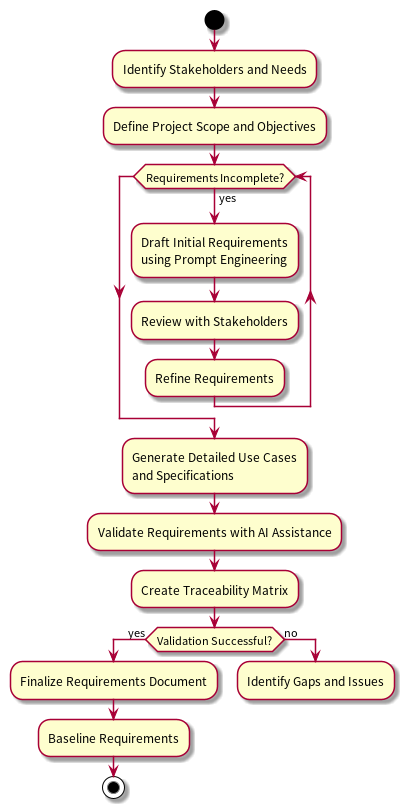
\includegraphics[width=0.3\textwidth]{images/re-pe.png} % Placeholder for PlantUML diagram
\end{frame}
\section{Case Study and Tools}

%%%%% \begin{frame}{Tool Integration}
%%%%%     \begin{columns}
%%%%%         \begin{column}{0.6\textwidth}
%%%%%             \textbf{Supported Tools:}
%%%%%             \begin{itemize}
%%%%%                 \item \textbf{AI Platforms}: ChatGPT, Claude, Gemini
%%%%%                 \item \textbf{RE Tools}: IBM DOORS, Jira, ReqView
%%%%%                 \item \textbf{Modeling}: PlantUML, Draw.io, Lucidchart
%%%%%                 \item \textbf{Version Control}: Git for prompt management
%%%%%                 \item \textbf{Validation Tools}: Custom scripts, AI evaluators
%%%%%             \end{itemize}
%%%%%         \end{column}
%%%%%         \begin{column}{0.4\textwidth}
%%%%%             \centering
%%%%%             \includegraphics[width=0.8\textwidth]{example-image} % Placeholder
%%%%%         \end{column}
%%%%%     \end{columns}
%%%%% \end{frame}

\begin{frame}[fragile]{Prompt Version Control Example}
    \lstset{style=code}
    \begin{lstlisting}[caption={Version-Controlled Prompt Template}]
# Prompt Template v2.1 - Use Case Generation
# Date: 2024-01-15 | Author: RE Team
# Changelog: Added validation criteria

SYSTEM_PROMPT: """
You are an experienced requirements engineer 
specializing in [DOMAIN]. Your task is to create 
comprehensive use case specifications.
"""

USER_PROMPT: """
Generate a use case for [FEATURE] in [SYSTEM] with:

1. PRIMARY_ACTOR: [actor role]
2. PRECONDITIONS: [system state requirements]
3. MAIN_SCENARIO: [step-by-step flow]
4. ALTERNATIVE_FLOWS: [error handling paths]
5. POSTCONDITIONS: [end state conditions]
6. VALIDATION: [acceptance criteria]

Format: Structured text with clear sections.
"""
    \end{lstlisting}
\end{frame}

\begin{frame}{Case Study: E-commerce System}
    \begin{block}{Project Overview}
        Developing an e-commerce platform using AI-assisted requirements engineering
    \end{block}
    
    \textbf{Results:}
    \begin{itemize}
        \item 40\% reduction in initial requirements gathering time
        \item 25\% fewer requirements defects identified during testing
        \item Improved stakeholder satisfaction with visual models
        \item Better traceability through structured prompts
    \end{itemize}
    
    \textbf{Challenges:}
    \begin{itemize}
        \item Training team on effective prompt engineering
        \item Integrating AI outputs with existing workflows
        \item Ensuring consistency across multiple AI sessions
    \end{itemize}
\end{frame}

\section{Conclusion and Future Directions}

\begin{frame}{Key Takeaways}
    \begin{itemize}
        \item \textbf{Synergy}: Prompt Engineering enhances traditional Requirements Engineering
        \item \textbf{Efficiency}: AI can accelerate requirements development and validation
        \item \textbf{Quality}: Structured prompts lead to better requirements specifications
        \item \textbf{Accessibility}: Visual models (like PlantUML) improve stakeholder understanding
        \item \textbf{Iterative Nature}: Both RE and PE benefit from continuous refinement
    \end{itemize}
    
    \begin{block}{The Future}
        AI will become an integral partner in requirements engineering, with prompt engineering as the essential interface between human intent and machine capability.
    \end{block}
\end{frame}

%%%%% \section{Research Topics in Requirements Engineering}

%%%%% \begin{frame}[t]{Research Topics in Requirements Engineering}
%%%%%     \begin{enumerate}
%%%%%         \item Requirements Classification
%%%%%         \item Requirements Prioritization
%%%%%         \item Feature Model Optimization
%%%%%         \item Prototype Generation
%%%%%     \end{enumerate}
%%%%% \end{frame}
%%%%% 
%%%%% \begin{frame}[t]{Techniques for Requirements Engineering Research}
%%%%% \end{frame}
%%%%% 
%%%%% \begin{frame}[t]{Next Release Problem}
%%%%%     % https://mde-optimiser.github.io/case-studies/nrp/
%%%%%     % https://www.sciencedirect.com/science/article/pii/S095058490100194X
%%%%%     % feature model
%%%%%     Given:
%%%%%     \begin{itemize}
%%%%%       \item A set of software requirements \( R = \{r_1, r_2, \dots, r_n\} \),
%%%%%       \item A set of customers \( C = \{c_1, c_2, \dots, c_m\} \),
%%%%%       \item Each customer \( c_j \in C \) requests a subset of requirements \( R_j \subseteq R \) and provides a profit  \( p_j > 0 \) if all requirements in \( R_j \) are satisfied,
%%%%%       \item Each requirement \( r_i \in R \) has an associated cost \( \text{cost}(r_i) > 0 \),
%%%%%       \item A total available budget \( B > 0 \).
%%%%%     \end{itemize}
%%%%% 
%%%%%     The goal is to select a subset of requirements \( R' \subseteq R \) such that:
%%%%%     \begin{enumerate}
%%%%%       \item The total cost does not exceed the budget: $\sum_{r_i \in R'} \text{cost}(r_i) \leq B$, 
%%%%%       \item The total profit is maximized:
%%%%%       \[
%%%%%       \max_{R' \subseteq R} \sum_{\substack{c_j \in C \\ R_j \subseteq R'}} p_j.
%%%%%       \]
%%%%%     \end{enumerate}
%%%%% 
%%%%%     This is known as the \textbf{Next Release Problem (NRP)} and is a well-known NP-hard problem in requirements engineering and software release planning.
%%%%% \end{frame}


\begin{frame}{References and Further Reading}
    \begin{thebibliography}{10}
        \bibitem{1} Sommerville, I. (2011) \emph{Software Engineering}
        \bibitem{2} Wiegers, K. \& Beatty, J. (2013) \emph{Software Requirements}
        \bibitem{3} White, J. et al. (2023) \emph{A Prompt Pattern Catalog to Enhance Prompt Engineering with ChatGPT}
        \bibitem{4} PlantUML Documentation (2024) \emph{Use Case Diagram Guide}
        \bibitem{5} Nuseibeh, B. \& Easterbrook, S. (2000) \emph{Requirements Engineering: A Roadmap}
    \end{thebibliography}
    
    \begin{center}
        \textbf{Thank You!}\\
        Questions?
    \end{center}
\end{frame}

\end{document}

